\documentclass[12pt, twoside]{article}
\documentclass[12pt, twoside]{article}
\usepackage[letterpaper, margin=1in, headsep=0.2in]{geometry}
\setlength{\headheight}{0.6in}
%\usepackage[english]{babel}
\usepackage[utf8]{inputenc}
\usepackage{microtype}
\usepackage{amsmath}
\usepackage{amssymb}
%\usepackage{amsfonts}
\usepackage{siunitx} %units in math. eg 20\milli\meter
\usepackage{yhmath} % for arcs, overparenth command
\usepackage{tikz} %graphics
\usetikzlibrary{quotes, angles}
\usepackage{graphicx} %consider setting \graphicspath{{images/}}
\usepackage{parskip} %no paragraph indent
\usepackage{enumitem}
\usepackage{multicol}
\usepackage{venndiagram}

\usepackage{fancyhdr}
\pagestyle{fancy}
\fancyhf{}
\renewcommand{\headrulewidth}{0pt} % disable the underline of the header
\raggedbottom
\hfuzz=2mm %suppresses overfull box warnings

\usepackage{hyperref}
\usepackage{float}

\title{Algebra 2}
\author{Chris Huson}
\date{January 2025}

\fancyhead[LE]{\thepage}
\fancyhead[RO]{\thepage \\ First \& last name: \hspace{2.25cm} \,\\ Section: \hspace{2.25cm} \,}
\fancyhead[LO]{BECA / Huson / Precalculus: Trigonometric functions \\* 9 April 2025}

\begin{document}

\subsubsection*{6.10 Quiz: The unit circle and cumulative year-to-date standards}
\begin{enumerate}[itemsep=0.5cm]
    \item Given a circle with radius of one, centered on the origin. An angle with measure $30^\circ$ is placed in standard position. 
    \begin{multicols}{2}
        \begin{enumerate}
            \item Mark the point $A$, the intersection of the circle and angle ray, as an ordered pair.            
            \item Write down the value of $\sin{30^\circ}$ \vspace{1cm}
            \item  Write down the value of $\cos{30^\circ}$
      \end{enumerate}
        
    \begin{center}
    \begin{tikzpicture}[scale=2.5]
      \draw[<->](-1.2, 0) -- (1.2, 0) node[above]{$x$};
      \draw[<->](0, -1.1) -- (0, 1.1);
      \draw(0, 0) circle[radius=1];
      \draw[->](0, 0) -- (30:1.2)node[below right] {$A=$};
      \fill(30:1.0) circle[radius=0.03];
      \node at (0.4,0.1){$30^\circ$};
      \draw(-1, 0) node[below left] {$(-1,0)$};
      \draw(1, 0) node[below right] {$(1,0)$};
    \end{tikzpicture}
    \end{center}
\end{multicols}

\item Convert each angle measure from degrees to radians or vice-a-versa.
    \begin{multicols}{2}
    \begin{enumerate}[itemsep=0.5cm]
        \item $60^\circ=$
        \item $\displaystyle \frac{\pi}{6}=$
    \end{enumerate}
    \end{multicols} \vspace{1cm}

\item For which angle measures $\theta$ is $\sin(\theta)$ negative? Select all that apply.
    \begin{multicols}{2}
    \begin{enumerate}[itemsep=0.5cm]
        \item $\pi$
        \item $\displaystyle \frac{3\pi}{2}$
        \item $\displaystyle \frac{7\pi}{4}$
        \item $\displaystyle \frac{\pi}{6}$
    \end{enumerate}
    \end{multicols} \vspace{1cm}

\item Given angle $A$ in the first quadrant with $\displaystyle \cos A=\frac{2}{\sqrt{5}}$, find the value of $\sin A$ in radical form.

\newpage
\item Simplify to standard form. \hfill \emph{A.APR.1 Perform operations with polynomials} \\[0.25cm]
$(7x^3 - 3x^2 + 3x - 3) - (2x^3 - 7x^2 - 5)$ \vspace{2cm}


\item Given $A = 3x^2-2$ and $B = 3x-4$, simplify $2A - B$. \vspace{5cm}

\item Write down the solutions to $3x(x + 1)(2x - 5) = 0$. \hfill \emph{A.APR.3 Find zeros of polynomials}
\vspace{2cm} 

\item Solve: $\displaystyle  x = \frac{4x-6}{x-1}$ \hfill \emph{A.REI.2 Solve rational and radical equations} \vspace{3cm} 

\item Solve for $x$ and check.
    \begin{multicols}{2}
    \begin{enumerate}[itemsep=0.5cm]
        \item  $\sqrt{x -2} + 5 = 8$
        \item Check your solution.
    \end{enumerate}
    \end{multicols}

\newpage
\item Write a recursive definition of the sequence \hfill \emph{F.BF.2 Sequences} \\[0.25cm]
$a_1 = 13$, $a_2 = 9$, $a_3 = 5$, $a_4 = 1, \ldots$ \vspace{2.5cm}

\item Simplify to the form $a+bi$ with $a,b$ real numbers. $x \in R$. \hfill \emph{N.CN.2 Complex numbers}
    \begin{multicols}{2}
        \begin{enumerate}[itemsep=1.5cm]
            \item $(x - 3i) - (2x - 2i)$
            \item $(5 - 3i)(2 + 3i)=$
        \end{enumerate}
    \end{multicols}  \vspace{5cm}

\item Simplify each expression, using imaginary numbers as necessary. $a > 0$
    \begin{multicols}{2}
    \begin{enumerate}[itemsep=0.5cm]
        \item $\sqrt{-49a^2}=$
        \item $\displaystyle \frac{3}{5} \sqrt{-50}=$
    \end{enumerate}
    \end{multicols} \vspace{1cm}
  
\item Rewrite each expression as a radical. \hfill \emph{N.RN.2 Radicals and rational exponents} \vspace{0.25cm}
    \begin{multicols}{2}
      \begin{enumerate}[itemsep=1cm]
        \item $\displaystyle 12^{-\frac{1}{2}}=$
        \item $\displaystyle (27x)^{\frac{2}{3}}=$
      \end{enumerate}
      \end{multicols} \vspace{1cm}
      
\item Rewrite each expression as a fractional exponent. $x>0$  \vspace{0.25cm}
    \begin{multicols}{2}
      \begin{enumerate}[itemsep=1cm]
          \item $\sqrt{7} =$
          \item $\sqrt[3]{x^6} =$
      \end{enumerate}
      \end{multicols}

\newpage
%F.LE.2.ii Construct an exponential function given a description.
\item Biologists are studying a new bacterium. They create a culture with 10,000 of the bacteria and anticipate that the number of bacteria will double every 5 hours. Write an equation for the number of bacteria, $B$, in terms of the number of hours, $t$, since the experiment began. %Jan 2020
    \vspace{2cm}

\item Graph the function $f(x) = 2x^{5}+3x^{4}-17x^{3}-12x^{2}+36x$. 
\begin{center}
    \begin{tikzpicture}[scale=0.65]
        \draw[lightgray,very thin] (-10,-10) grid (10,10);
        \draw [thick,<->] (-10.5,0)--(10.5,0) node [right] {$x$};
        \draw [thick,<->] (0,-10.5)--(0,10.5) node [above] {$f(x)$};
        \foreach \x in {2}
            \draw[thick] (\x cm,5pt) -- (\x cm,-5pt) node[below] {$1$};
        \foreach \y in {2}
            \draw[thick] (4pt,\y cm)--(-4pt,\y cm) node[left]{10};
    \end{tikzpicture}
    \end{center}
Mark and label the zeros of the function. \\[0.25cm]
Describe the behavior of the given function as $x$ approaches positive infinity.


\newpage

\item The polynomial $f(x)=x^3-13x-12$ is shown on the graph below. What is the slope between the local minimum at $x=2$ and the $x$-intercept at $x=4$? This is called the \emph{average rate of change} between $x=2,4$.
\begin{center}
    \begin{tikzpicture}[scale=2.25/4]
    \draw[step=1cm,gray,very thin] (-7,-7) grid (7,7);
    \draw[thick,<->] (-7.5,0) -- (7.5,0) node[anchor=north west] {\textbf{x}};
    \draw[thick,<->] (0,-7.5) -- (0,7.5) node[anchor=south east] {\textbf{y}};
    \foreach \x in {-6, -4, -2, 2, 4, 6} \draw (\x cm,1pt) -- (\x cm,-1pt) node[anchor=north] {$\x$};
    \foreach \y in {-3} \draw (1pt,\y cm) -- (-1pt,\y cm) node[anchor=east] {$-30$}; %{$\y$};
    %\tkzInit[xmin=-6,xmax=5,ymin=-7,ymax=7,ystep=1]   
    %\tkzFct[color=black,thick,<->,domain = -4.3:4.9] {0.1*(x+3)*(x+1)*(x-4)};
    \draw [thick, <->, smooth,domain=-4.3:4.9] plot(\x,{0.1*(\x+3)*(\x+1)*(\x-4)}) node[below right]{$f$};
    \draw [dashed] (2,-3) -- (4,0);
    \end{tikzpicture}\\*[1.5in]
\end{center}

\item The graph shows the exponential function $\displaystyle f(x)$.
\begin{multicols}{2}
    \begin{enumerate}[itemsep=1cm]
        \item Write down the initial value of the function.
        \item By what factor do the values of $f$ increase each time $x$ increases by 1?
        \item Write an expression for the function $f(x)$.
    \end{enumerate}
    \begin{center}
    \begin{tikzpicture}[x=1cm, y=0.15cm, xscale=2]
        \draw [thin, color=lightgray, xstep=0.5cm,ystep=0.75cm] (0,0) grid (3,40);
        \draw [thick, ->] (0,0) -- (+3.3,0) node [below]{$x$};
        \draw [thick, ->] (0,0) -- (0,43) node [right]{$y$};        
        \foreach \x in {0,0.5,...,3}
            \draw (\x cm,0) -- (\x cm,0) node[below] {$\x$};
        \foreach \y in {0,10,20,...,40}
            \draw[shift={(0,\y)}] (2pt,0pt)--(-2pt,0pt) node[left]{$\y$};
        \draw [thick, ->, smooth,domain=0.:2.6] plot(\x,{10*(1.732^\x)}) node[below right]{$f$};
        \fill (0,10) ellipse [x radius=1pt, y radius=2pt]  node [below right] {$(0,10)$};
        \fill (2,30) ellipse [x radius=1pt, y radius=2pt] node [below right] {$(2,30)$};
    \end{tikzpicture}
    \end{center}
    \end{multicols} \vspace{1cm}

\item Graph the continuous exponential function $f(x) = 3e^{0.08x}$ on the grid below. 
\begin{center}
    \begin{tikzpicture}[scale=1]
        \draw[gray,thin] (0,0) grid (10,10);
        \draw [thick,->] (0,0)--(10.5,0) node [right] {$x$};
        \draw [thick,->] (0,0)--(0,10.5) node [above] {$f(x)$};
        \foreach \x in {0,1,...,10}
            \draw (\x cm,5pt) -- (\x cm,-5pt) node[below] {$\x$};
        \foreach \y in {0,1,...,10}
            \draw[shift={(0,\y)}] (2pt,0pt)--(-2pt,0pt) node[left]{$\y$};
    \end{tikzpicture}
    \end{center}
    \begin{enumerate}
        \item Graph the line $y=6$. Mark the intersection of the line with $f$ and label it as an ordered pair, rounded \emph{the nearest whole number}.
        \item The function $f(x)$ models the growth of an investment. Explain what the values of $3$ and $0.8$ represent in the context of the investment. \vspace{4cm}
        \item How long will the investment take to double? 
    \end{enumerate}
       
\end{enumerate}
\end{document}